\documentclass[]{final_report}
\usepackage{graphicx}
\usepackage{hyperref}
\usepackage{listings}
\usepackage{svg}
\usepackage{afterpage}
\usepackage{pdflscape}
\usepackage{listings}
\usepackage{amsmath}

\lstset{basicstyle=\ttfamily}
\usepackage{color}
\definecolor{lightgray}{rgb}{.9,.9,.9}
\definecolor{darkgray}{rgb}{.4,.4,.4}
\definecolor{purple}{rgb}{0.65, 0.12, 0.82}
\lstdefinelanguage{JavaScript}{
  keywords={break, case, catch, continue, debugger, default, delete, do, else, false, finally, for, function, if, in, instanceof, new, null, return, switch, this, throw, true, try, typeof, var, void, while, with},
  morecomment=[l]{//},
  morecomment=[s]{/*}{*/},
  morestring=[b]',
  morestring=[b]",
  ndkeywords={class, export, boolean, throw, implements, import, this},
  keywordstyle=\color{blue}\bfseries,
  ndkeywordstyle=\color{darkgray}\bfseries,
  identifierstyle=\color{black},
  commentstyle=\color{purple}\ttfamily,
  stringstyle=\color{red}\ttfamily,
  sensitive=true
}

\lstset{
   language=JavaScript,
   backgroundcolor=\color{lightgray},
   extendedchars=true,
   basicstyle=\footnotesize\ttfamily,
   showstringspaces=false,
   showspaces=false,
   numbers=left,
   numberstyle=\footnotesize,
   numbersep=9pt,
   tabsize=2,
   breaklines=true,
   showtabs=false,
   captionpos=b
}

%%%%%%%%%%%%%%%%%%%%%%
%%% Input project details
\def\studentname{Arran France}
\def\reportyear{2018}
\def\projecttitle{Array Support for Dynamic Symbolic Execution of JavaScript}
\def\supervisorname{Dr Johannes Kinder}
\def\degree{BSc (Hons) in Software Engineering}
\def\fullOrHalfUnit{Full Unit} % indicate if you are doing the project as a Full Unit or Half Unit
\def\finalOrInterim{Final Report} % indicate if this document is your Final Report or Interim Report

\begin{document}

\maketitle

%%%%%%%%%%%%%%%%%%%%%%
%%% Declaration

\chapter*{Declaration}

This report has been prepared on the basis of my own work. Where other published and unpublished source materials have been used, these have been acknowledged.

\vskip3em

Word Count: 

\vskip3em

Student Name: \studentname

\vskip3em

Date of Submission: 

\vskip3em

Signature:

\newpage

%%%%%%%%%%%%%%%%%%%%%%
%%% Table of Contents
\tableofcontents\pdfbookmark[0]{Table of Contents}{toc}\newpage

%%%%%%%%%%%%%%%%%%%%%%
%%% Your Abstract here

\begin{abstract}

This will be written the day before the submission.

\end{abstract}
\newpage

%%%%%%%%%%%%%%%%%%%%%%
%%% Introduction
\chapter{Introduction}
%%%%%%%%%%%%%%%%%%%%%% // TODO REWORK, CITE, AND PROOF READ
Since its inception as a `glue' language for the web, JavaScript's popularity has surged, it's now a ubiquitous language that powers mobile, web, and server applications, however its dynamic nature and deceptive syntax often lead to subtle bugs and unintended behaviour which can be difficult to identify. Dynamic symbolic execution (DSE) is a technique that can be used to automatically identify bugs and generates tests for JavaScript however this requires modelling the semantics of the language in first order logic. JavaScript arrays, in particular, are an area of the language that requires tradeoffs, difficult design decisions, and careful consideration of language semantics when modelling due to their atypical properties. JavaScript arrays are special cases of objects and as a result have a settable length, can consist of multiple types, and are not necessarily indexed sequentially.

My work extends ExpoSE, a tool for DSE, by describing an encoding for homogeneously typed JavaScript arrays in first order logic, implementing support in ExpoSE for symbolic arrays, and modelling a selection of prototype functions. I demonstrate that as a result of these extensions results in an increased test coverage of popular several popular JavaScript libraries and describe a new bug found in a popular Array ES6 polyfill. I also describe some of the limitations and 

I also present background information on symbolic execution, including considerations for constraint optimisations and its usage for bug detection, automated decision procedures, and JavaScript's semantics, with a particular focus on the behaviour of arrays and their prototype methods. I then describe the details of implementation, my experimental methodology, and conclusions.

%%%%%%%%%%%%%%%%%%%%%%
%%% Symbolic Execution
\chapter{Symbolic Execution}

%%%%%%%%%%%%%%%%%%%%%% Overview
\section{Overview}

Symbolic execution is a technique for testing program correctness initially proposed in the 1970s~\cite{king1976symbolic, boyer1975select}. Classically, it is the process of executing a program by representing its variables as symbols rather than concrete values. Execution of the program occurs using these symbolic inputs by extending the basic operators and semantics of the program's language to use symbols and produce symbolic formulas rather than concrete values. In doing so, each symbolic execution tests many actual instances of execution. If statements and language features that cause execution to diverge are represented as a path condition, a conjunction of conditions on symbols that must be satisfied. At the end of execution the path condition, the conjunction of branch conditions taken to the current point of execution, provides a unique representation of a path tested through the program and when solved using a constraint solver produces a set of inputs that when run take the same path through the program as the symbolic execution~\cite{godefroid2008automated, godefroid2005dart}.

\begin{figure}[h]
\begin{lstlisting}
function abs_sum (x, y) {
 if (x < 0) {
   x = x * -1;
 }
 if (y < 0) {
   y = y * -1;
 }
 return x + y;
}
\end{lstlisting}
\caption{\label{fig:abs-sum} Absolute Sum Function}
\end{figure} 

For example, consider the program described in Figure \ref{fig:abs-sum} which returns the sum of the absolute values of two values. There are four possible paths that can be taken through the program. The first is where neither if branches are entered, the second is where the value of \lstinline{x}  is less than zero, the third is where the value of \lstinline{y} is less than zero, and the fourth is where both \lstinline{x}  and \lstinline{y} are less than zero. The process for symbolically executing this program classically is as follows. The function is executed with two symbolic values $x'$ and $y'$ and a path condition $pc$, "the accumulator of properties which inputs must satisfy ... to follow ... a particular path"~\cite{king1976symbolic}, is initialised to $true$. When a branching statement (line 2 or 5) is reached the constraint solver is queried to see if the branch condition is feasible given the current path condition. If condition is satisfiable then execution forks to explore the new path and $pc$ becomes $pc \land bc$  where $bc$ is the branch condition. This process repeats until the program terminates and every path is explored. Table \ref{abs-sum-se-table} shows the path condition, symbolic results, and the constraint solver queries and results for the execution.

\begin{table}[]
\centering
\begin{tabular}{|l|l|l|l|}
\hline
$pc$                & Result  & Constraint Solver Queries & Query Result \\ \hline
$x >= \land y >= 0$ & $x+y$   & $x >=0 \land y < 0 $      & SAT          \\ \hline
$x >= \land y < 0$  & $x - y$ & $x <0 $                   & SAT          \\ \hline
$x < \land y >= 0$  & $-x+y$  & $x<0 \land y < 0 $        & SAT          \\ \hline
$x < \land y < 0$   & $-x-y$  &                           &              \\ \hline
\end{tabular}
\caption{Absolute Sum Symbolic Execution Results}
\label{abs-sum-se-table}
\end{table}

Historically, this technique has been impractical due to the limitations on computing resources and the capabilities of automated theorem provers~\cite{king1976symbolic}. However in the 2000s there were a a number of advancements in the technique by DART~\cite{godefroid2005dart} and EXE~\cite{cadar2008exe} which combined with improvements in computer hardware and SMT solvers~\cite{de2011satisfiability} made the technique practical.

In these modern implementations, the program is run both concretely and symbolically in so called concolic execution. In concolic execution, the program is instrumented to run concretely whilst the program state is shadowed by symbolic variables allowing the concrete execution to`drive' the symbolic execution. Unlike pure symbolic execution, concolic execution requires its initial input to be concrete, this input can be random or crafted to fit the target program~\cite{godefroid2008grammar,cadar2013symbolic}. As concolic execution concretely executes programs, rather than just modelling the semantics of the language, you can be sure that any bugs found are actual bugs. Additionally, when a constraint cannot be solved, concolic execution allows concrete values to be substituted for unsolvable elements of constraints~\cite{sen2007concolic,sen2005cute}.

Consider the following example of concolic execution testing the program described in  Figure~\ref{fig:abs-sum}. Inputs for \lstinline{x} and \lstinline{y} are randomly generated, for instance $x=217$ and $y=931$. These then guide the execution to not visit any branches, producing the $pc$ of $x >= 0 \land y >=0$. This path condition can then be negated to produce further paths. Using the DART~\cite{godefroid2005dart} style directed symbolic execution paths are generated as per Table~\ref{abs-sum-ce-table}.

\begin{table}[]
\centering
\begin{tabular}{|l|l|l|l|l|}
\hline
Input (x, y) & $pc$ & Result & Constraint Solver Queries & Query Result \\ \hline
0, 0 & $x >= \land y >= 0$ & $x+y$ & $x >=0 \land y < 0 $ & SAT \\ \hline
0, -3 & $x >= \land y < 0$ & $x - y$ & $x <0 $ & SAT \\ \hline
-2, 1 & $x < \land y >= 0$ & $-x+y$ & $x<0 \land y < 0 $ & SAT \\ \hline
-2, -7 & $x < \land y < 0$ & $-x-y$ &  &  \\ \hline
\end{tabular}
\caption{Absolute Sum Concolic Execution Results}
\label{abs-sum-ce-table}
\end{table}


%%%%%%%%%%%%%%%%%%%%%%  Finding and Choosing Paths
\section{Finding and Choosing Paths}

Although, in theory, symbolic execution will exhaustively search through all feasible paths, as the length of the program under test increases the number of paths in the program increases roughly exponentially~\cite{cadar2013symbolic}. As these symbolic execution tools are bounded by real world time constraint, paths must be chosen carefully in order to prioritise exploring `interesting' cases in the time available.

In EXE, and other more traditional methods, paths are found by building a control flow graph and then exploring the graph using a form of breadth-first search (BFS) or depth-first search base. Neither BFS or DFS are particularly well suited for the problem as neither is able to prioritise`interesting paths', they simple try to exhaustively explore all the paths in a program. DFS is especially flawed due to its ability to get `stuck' in a symbolically bounded loop~\cite{cadar2008exe}. 

SAGE, by contrast, uses a \textit{generational search}. Following the initial input, paths are generated by repeatedly negating the conditions in the path condition that was explored. Then paths are prioritised using a priority queue~\cite{godefroid2005dart}.

In detail, the algorithm for finding new test inputs is as follows: starting with an initial input $i$ which has an attribute, $bound$ of 0, and a priority queue $pq$ the program executes symbolically and returns the path condition for its execution, $pc$, in the form of a sequence of predicates $c_1 \land c_2 \land ... c_n $.  To explore alternatives to the branches that were chosen in the last execution, for $j = i.bound ... n$ where $n$ is the number of predicates in $pc$,  new inputs are generated by negating the $c_j$ and solving the new constraint~\cite{godefroid2005dart, godefroid2008grammar}. Each new input is pushed to $pq$ with a bound of $j$. $bound$ is used to prevent path conditions being explored multiple times. The paths in the priority queue can then be prioritised using a chosen heuristic~\cite{cadar2013symbolic}. 

Constraint solvers are used for two purposes in symbolic execution: determining the satisfiability of branch/path constraints and producing concrete input for satisfiable conditions. Despite continual improvements in the performance of constraint solvers, calls to solvers are typically the bottleneck is symbolic execution - fortunately there are a number of possible optimisations that can be done to reduce the burden on constraint solvers and achieve better performance~\cite{cadar2013symbolic}.

%%%%%%%%%%%%%%%%%%%%%%  Finding and Choosing Paths
\section{Constraint Optimisations}
Frequently constraints will need to be solved multiple times throughout the course of execution. Instead of calling the constraint solver multiple times for the same constraint, satisfying results can be stored in a map of constraints to satisfying results. Then, instead of directly calling the constraint solver directly, a cache lookup can be performed first to see if there is a satisfying result~\cite{cadar2008klee}.

This caching process can be extended to evaluate the strength of formulas. If there is a satisfying result for a stronger constraint than the one being queried then that satisfying result will be valid for the weak constraint. For instance, if the cache contains the following mapping $ (x > 3 \land y <1) \land (x < 10) \implies x = 5 \land y =  -214$ then the satisfying result will be valid for the condition $x > 3 \land y < 1 $ . This caching scheme can also be used to cache unsatisfiable constraints~\cite{cadar2008klee}.

In most cases, a branch's condition will not depend on all of the variables in a path constraint allowing redundant constraints to be eliminated before passing the constraint to constraint solver. Although if this technique is applied the constraint solver will only return satisfiable values for non-eliminated variables, the existing concrete values of the other variables can be used to produce a full set of inputs~\cite{cadar2013symbolic}.

For instance, consider the function in figure 2.2. If the existing path constraint is  $(x < 0 ) \land ( z  > 5) \land (y < 13) \land (y + x > 15) $ and the symbolic execution negates the the last path condition to explore a new path:  $ (x < 0) \land (z > 5) \land (y < 13) \land \lnot(y + x > 15)$ then the  $z > 5$ constraint can be eliminated as $z$ does not influence the $y + x > 15$ branch.

\begin{figure}[h]
\begin{verbatim}
function unlikely_function (x, y, z){
 if (x < 0)
   x--
 if (z > 5)
   z++
 if (y < 13)
   y++
 if (y + x > 15)
   y = y * x
 return x + y + z
}
\end{verbatim}
\caption{\label{fig:example-function} Example Function}
\end{figure} 

\section{Bug Detection}

Symbolic execution can be used for a variety of purposes, for instance: generating test inputs, finding infeasible paths,  finding equivalent (and therefore redundant code) but its typical application, and the focus of this project, is bug detection. 

In classical symbolic execution, as no actual code is executed bugs must be detected through the use of logical assertions that are tested by the constraint solver.  EFFIGY, described in~\cite{king1976symbolic} uses the concept of an input predicate and an output predicate to determine program correctness. If for all inputs which satisfy the input predicate also satisfy the output predicate then the program is said to be correct. These are implemented through the use of \lstinline{ASSERT}, \lstinline{ASSUME}, and \lstinline{PROVE} statements. In modern symbolic execution tools such as DART, rather than having to add additional assertions bugs are detected when runtime exceptions occur ~\cite{godefroid2005dart}.

Symbolic execution offers a number advantages over typical testing techniques. Unit and integration testing are expensive and require a large amount of effort to reach 100\% coverage. In addition, they require a large amount of mock and driver code to be written, often exceeding the size of the program under test. Unit testing and integration often miss `corner case' bugs, which are not considered either when the program is developed or when the system is tested.

Static analysis is much cheaper to run but at the cost of precision. Static analysis often produces false reports and consequently also requires a large amount of time spent to identify actual faults. Static analysis often may struggle to identify subtle bugs due to the lack of information available outside of runtime, and will typically perform worse on weakly typed languages.

Symbolic execution, like static analysis, requires no additional effort on the part of the developer and has the advantage of not producing false positives and providing a valid test case for each bug found. Symbolic execution is also effective at finding edge case bugs and can also effectively analyse the behaviour of a program when it interacts with libraries.

\chapter{Automated Decision Procedures}

\section{A Short History of Automated Reasoning}
The notion of automated reasoning has long existed, the most prominent early example being Gottfried Leibniz's dream of a machine which could automatically determine the truth of any assertion, ``If controversies were to arise, there would be no more need of dispute between two philosophers than between two accountants". Leibniz's dream was later echoed in David Hilbert's challenge to the 1928 International Congress of Mathematicians, known now as the \textit{Entscheidungsproblem} or decision problem, in which he posed the question (paraphrased here) ``Is there a mechanical procedure which when fed any mathematical proposition determines in a finite number of steps whether or not the statement is provable from a set of axioms, using first-order logic?"~\cite{smtwheredowegofromhere, automatedreasoningbooklet2004}.

At the time Hilbert proposed his challenge no formal notion of a mechanical procedure, or algorithm, existed. In 1935/6 Alonzo Church and Alan Turing independently defined equivalent notions of an algorithm, lambda calculus and Turing machines, and found a negative result for the \textit{Entscheidungsproblem}  by proving that first-order logic is undecidable~\cite{turingchurchproof}.

Despite first-order logic being generally undecidable, there are some first order theories which are including Presburger Arithmetic, a first order theory of only addition over natural numbers - more limited than the general undecidable Peano's arithmetic~\cite{automatedreasoningbooklet2004}. In 1954, Martin Davis implemented a decision procedure for Presburger arithmetic producing the first computed mathematical proof. He remarked later, ``Its great triumph was to prove that the sum of two even numbers is even," an acknowledgement of the achievement of the program but also its limitations~\cite{excapebarrettriseofsmt, automatedreasoningbooklet2004}.

From the 1950s onwards there was a steady increase in the body of work related to automated reasoning including work by Davis and Putman ~\cite{Davis:1960:CPQ:321033.321034} ~\cite{Davis:1962:MPT:368273.368557}, John Robinson's proof of the soundness and completeness of first order resolution ~\cite{robinson1965machine}, and Simon and Newell's Logic Theorist ~\cite{newell1956logic} however this drastically accelerated took off in 2000s following the publication of the Chaff SAT solver~\cite{moskewicz2001chaff} and a renewed interested in theory solving~\cite{excapebarrettriseofsmt}.

\section{SAT}
A classic problem in the realm of automated reasoning is the SAT problem. The SAT problem asks the question ``Given a formula in propositional logic is there an assignment of true/false values that makes the formula true?"~\cite{smtwheredowegofromhere}.

For instance, given for the following formula, the answer would be no, the problem is unsatsifiable:,  $(a \lor b) \land (b \land \lnot a) \land \lnot b $.

In the 1970s, Stephen Cook and Leonid Levin showed the SAT problem was NP-complete seeming to make automated reasoning infeasible for efficient algorithms. However, although random SAT problems exhibit worst-case performance, many real-world problems tend not to due to their tendency to have structure~\cite{smtwheredowegofromhere}.

Most SAT solvers, automated tools to produce solutions for a given SAT problem, use the Davis-Putnam-Logemann-Loveland (DPLL) backtracking search combined with Conflict-Driven-Clause-Learning (CDCL) to determine satisfiability~\cite{zhang2001efficient, gomes2008satisfiability}.

\subsection{DPLL}
DPLL is a depth-first search complete systematic process for finding a satisfying assignment or proving unsatisfiability for a given SAT problem.  The algorithm, at first approximation, attempts to assign a variable a Boolean value, and checks the satisfiability of the problem (with the assigned values). If the problem is not unsatisfiable then another variable has a value assigned, otherwise the previously assigned value is negated. This process is repeated until all variables are assigned a value and either the formula is satisfiable or, no matter what variable is assigned, a value the formula is unsatisfiable~\cite{sattosmt}.

Typically SAT problems are expressed in conjunctive-normal form (CNF), as a conjunction of one or more clauses which consist of the disjunction of one or more literals.

It is possible to model the algorithm as a series of states and transitions. States are described in the form $M || F$, where $M$ is a sequence of literals which are assigned the value true and $F$ is the problem in CNF form. The initial state of the algorithm is as $\emptyset || F $ and the final is state is either a special state $unsat$ if $F$ is unsatisfiable, or $M || G $, where $G$ is a CNF formula equivalent to the initial problem $F$ and $M$ satisfies $G$. 

The transitions between states are described by a number of rules as described in Table \ref{dpll-rules}. $M \models C$  means that for every assignment $v$, $v(M) = true$ implies $v(C) = true$. These rules are applied to each state until a final state is achieved.

\afterpage{%
    \clearpage% Flush earlier floats (otherwise order might not be correct)
    \begin{landscape}% Landscape page
\begin{table}[]
\centering
\caption{DPLL Rules}
\label{dpll-rules}
\scalebox{.60}{
\begin{tabular}{|l|l|l|l|}
\hline
Name & Rule & Conditions & Example \\ \hline
Unit Propagation & $M|| F, C \lor l \implies M l || F, C \lor l$ & ​$M \models \lnot C $,  $l$ is undefined in $M$ & $\emptyset || a \land (b \lor c) ) \land (d \lor e) \implies a || a \land (b \lor c) ) \land (d \lor e) $ \\ \hline
Pure Literal & $M|| F \implies Ml || F$ & $l$ occurs in some clause of $F$, $\lnot l$ occurs in no clause of $F$, $l$ is undefined in $M$ & $\emptyset || a \land (\lnot b \lor c) \implies \lnot b ||,a \land (\lnot b \lor c) $ \\ \hline
Decide & $M|| F \implies M l^d || F$ & $l$ or $\lnot$ occurs in a clause of $F$ & $ \lnot b |  \lnot b ||, a \land (\lnot b \lor c) \implies\lnot b \land c^d ||,a \land (\lnot b \lor c) $ \\ \hline
Fail & $M|| F, C \implies unsat$ & $M \models \lnot C$ $M$ contains no decision literals ($l^d$) & $ a \land \lnot a || \lnot a \land a \implies unsat $ \\ \hline
Backjump & $M l^d N|| F, C \implies M l' || F, C$ & $M l^d N \models \lnot C$ and there is a clause $C' \lor l'$ where $F, C \models C' \lor l'$ and $M \models \lnot C'$, $l'$ is undefined in $M$, and $l' or \lnot l'$ occurs in $F$ or in $M l^d N$ & TODO \\ \hline
Learn & $M|| F \implies,M || F, C$ & All atoms of $C$ occur in $F$, $F \models C$ &  \\ \hline
Forget & $M|| F, C \implies M || F $ & $F \models C$ &  \\ \hline
Restart & $M|| F \implies \emptyset || F$ &  &  \\ \hline
\end{tabular}
} %end scale
\end{table}
\end{landscape}
    \clearpage% Flush page
}

\subsection{CDCL}
As variables are assigned Boolean values during the DPLL algorithm, conflicts arise from the implications of such assignments. For instance consider the following problem in CNF:

$(a \lor b \lor \lnot c) \land (a \lor \lnot d) \land (c \lor d \lor e) \land (\lnot e \lor \lnot f ) \land (g \lor \lnot e \lor \lnot h) \land (f \lor h)$

With the assignments $g = \mathit{false}$, $a = \mathit{false}$, and $b = \mathit{false}$ the last clause, $ (f \lor h) $,  becomes unsatisfiable as $ f = \mathit{false}, h = \mathit{false}$ is implied.

CDCL attempts to identify the reason for the conflict and then use that information to jump several decisions back in the search to try a new assignment that will avoid that conflict. This process avoids exploring search spaces where there cannot be a solution. 

In DPLL with CDCL, each assignment has a 'decision level' which represents the number of assignments away from the start the algorithm is. As the procedure assigns values to variables, a graph of the assignments and their implications can be built. When a conflict arises, a bipartition of the graph identifies the conflicting variables and the assignment that caused the implication. The way this information is stored and used for future assignments is implementation dependent but following the conflict, the algorithm will back track to the decision level before the assignment that caused the implication and will resume.

\section{SMT}

SMT solvers combine SAT solving with theory specific reasoning in order to tackle problems beyond simple Boolean formulas. While SAT solver problems are defined exclusively in propositional logic, SMT problems can be defined using first-order logic for any theories that the SMT solver supports. Commonly supported theories include the theory of uninterpreted functions, equality, bit vectors,  arithmetic, and arrays. In practice these solvers look a lot like the automated reasoning machines that Hilbert and Leibniz imagined and can be applied to many domains such as program verification, scheduling, exploit generation, AI planning, and network analysis.

SMT solvers can be classified into two distinct types: eager solvers and lazy solvers. Eager solvers attempt to transform the theory expression into a Boolean formula that can be passed to the SMT solver's underlying SAT solver. Lazy solvers instead rely on their theory solvers and pass information between the theory solvers and the SAT solver. Although eager solvers, or bit blasters, are still commonly used for problems that manipulate bit-vectors most SMT solvers now use lazy solving. Lazy solvers attempt to take advantage of the domain specific strength of the theory solvers and rely only on the SAT solver for the skeleton Boolean formula reducing by avoiding reasoning about the entire formula~\cite{sattosmt, smtdpplt}.

The adjustments that must be made to the state transition model of DPPL are as follows. 

The final state is either $unsat$ or $M || F$ and $Solv _T(M)$ is satisfiable, where $Solv_T$ is a theory solver that can check theory satisfiability for $F$.

We also have to amend the Theory Learn and Forget rules to prevent being stuck in a state where $M || F, M \models F$, and $Solv_T(M)$ is not satisfiable by ensuring that the backtrack rule can be applied. The backtrack rule has a condition that $M \models \lnot C$. In this unsatisfiable state $T \models \lnot M$ so any clause for which $T \models C$ will enable backtracking. Finally, the pure literal rule needs to be removed. Although in Boolean logic literals are independent of each other in first-order this may not be the case.


\begin{table}[h]
\centering
\caption{SMT Rules}
\label{smt-rulesl}
\begin{tabular}{|l|l|l|}
\hline
Name & Rule & Conditions \\ \hline
Theory Learn & $M || F \implies M|| F, C $ & All atoms of $C$ occur in $F$, $F \models _T C $ \\ \hline
Theory Forget & $M || F, C \implies M || F $ & $F \models _T C$ \\ \hline
\end{tabular}
\end{table}

\subsection{Example Lazy Approach}
Consider the problem below which uses the theory of equality of uninterpreted functions (EUF).

$ f(a) = b \land  (g(f(c)) \neq g(b) \lor g(a) = g(b)) \land a \neq c $

The SAT solver runs on the Boolean skeleton of the formula $1 \land (2 \lor 3) \land 4$ and suggests a model $M$, $1 = \mathit{true}, 2 = \mathit{false}, 3 = \mathit{true}, 4 = \mathit{true}$. The theory solver then finds the theory inconsistent, and adds a negation of the inconsistent model to the model preventing that state from being explored again - this new model $ 1 = \mathit{true}, 2 = \mathit{false}, 3 = \mathit{true}, 4 = \mathit{true}, (\lnot 1 \lor 2 \lor \lnot 3 \lor 4 ) = true $  is then solved by the SAT solver to produce a new model $ 1 = \mathit{true}, 2 = \mathit{true}, 3 = \mathit{false}, 4 = \mathit{true}$. This model is then sent to the theory solver which finds the theory consistent producing a satisfiable result.

This basic lazy approach works well as it focuses on the domain specific strengths of the SAT solver and theory solver and it allows the SMT solver to be built modularly as the SAT and theory solvers communicate via a simple interface. Replacing the theory or SAT solver can be done independently from each other. However this basic lazy approach, even optimised, doesn't use any theory information to guide the search~\cite{sattosmt}.

\subsection{DPPL(T)}
Rather than simply validating models suggested by the SAT solver, DPLL(T) uses the theory solver to find T-consequences to guide the search. It produces explanations of inconsistent states and is able to backtrack to known good states to continue search~\cite{smtdpplt, ganzinger2004dpll}.

DPLL(T) adds a new rule T-Propagate which is described as $M || F \implies M l || F $ under the conditions $M \models _T l$, $l$ or $\lnot l$ occurs in $F$, and $l$ is undefined in $M$~\cite{sattosmt}.

When a non-Boolean conflict occurs then the theory solver provides a conjunction, $E$, of inconsistent literals were in the model when it was found to be inconsistent.  For each literal $e $ in $E$, if $e_1$ was T-propagated then a reason for the inconsistency can be described as another set of literals $R$ where $r_1 \land ... \land r_n \models _T e$. 

\subsection{Combining Theory Solvers}
In many cases problems cannot be simply modelled by a single theory. For instance, in the of modelling arrays we require at least the theory of arrays and the theory of arithmetic. It may be possible to use the union of the theories using the Nelson-Oppen combination~\cite{smtdpplt}.

Given two disjoint theories $T_1$ and $T_2$, where the theories are stably-infinite and convex, and a set of literals $S$ the deterministic Nelson-Oppen algorithm has the following steps.

1. Purify each literal in $S$ so that it belongs to a single theory, $S_1$ or $S_2$ where $S = S_1 \bigcup S_2$

2. Agree constants for each literal in $S$ and exchange equalities $E$, between $S_1$ and $S_2$

3. Check the satisfiability of each equality $e$ in $E$ with the corresponding solver If any unsat, report unsat - else report sat.

For instance consider the set of literals $f(a) - f(b) = c, c = a -5, f(0) = 3, a = b$ and the theories of arithmetic and equality of uninterpreted functions.

\textbf{Steps 1 and 2}

$f(a) - f(b) = c \implies f(a) = t_1, f(b) = t_2, c = t1 - t2$

$c = a - 5 \implies t_5 = a - 5 \implies t_5 = t_3, t_3 = a- 5$

$f(0) =3 \implies f(t_4) = t_5, t_4 = 0, t_5$

The solvers share constants: $t_1$ .... ,$t_5, a, b, c$.

\textbf{Step 3}

For each literal, its theory solver checks the satisfiability. In this example, each theory returns satisfiable.

\chapter{JavaScript}

JavaScript was initially created by a team at Netscape in 1996 with the goal of bringing interactivity to the web via a scripting language. According to Brendan Eich (the creator of JavaScript), up until this point the web was ``static, text-heavy, with at best images in tables or floating on the right or left"~\cite{AZProgrammingLanguages}. 

Brendan was initially recruited by Netscape with the aim of implementing Scheme, a dialect of Lisp that supports first-class functions~\cite{dybvig1996scheme}, in the browser however by this time Sun and Netscape were negotiating to bring Java to Netscape Navigator~\cite{popularityofjavascript}. An internal debate occurred about the need for two languages but Eich and other influential developers at both Sun and Netscape believed that the two languages would serve different audiences. 'Professional' developers would veer towards Java for building logic heavy components and designers and amateurs would use the scripting language as a `glue' for joining together components~\cite{AZProgrammingLanguages}.

Despite targeting a different audience Mocha, the language that would later evolve into JavaScript, was required by management to ``look like Java", according to Eich, ruling out the existing languages Perl, Python, and Scheme. Eventually Eich settled on ``Scheme-ish first-class functions and Self-ish (albeit singular) prototypes as the main ingredients"~\cite{popularityofjavascript}. Mocha also inherited a number of confusing Java language features such as the distinction between primitives and objects (e.g.\lstinline{string}vs.\lstinline{String}) and the\lstinline{Date}constructor which is a port of Java's\lstinline{java.util.Date}, complete with the Y2K bug~\cite{brendaneichtimetomakejscomment}. Perl and Python are also credited to influencing Mocha's string handling and regular expressions and AWK inspired the use of the\lstinline{function}keyword briefhistoryofjavascript. The first version of the language had an incredibly short development period. Eich claims he spent ``about ten days" developing the first JavaScript interpreter~\cite{AZProgrammingLanguages}.

After JavaScript (abandoning its previous names, Mocha and LiveScript) was released in Netscape Navigator 2 Microsoft began work on JScript, an equivalent language which shipped with Internet Explorer 3. Eich says that ``At some point in late summer or early fall 1996, it became clear to me that JS was going to be standardized. Bill Gates was bitching about us changing JS all the time."~\cite{newjavascriptmoduleowner} This led to JavaScript being standardised by Ecma International, an industry group that produces information standards, as ECMAScript in 1997. Since 1997 ECMAScript, now in its sixth version, has also been adopted as an ISO/IEC standard~\cite{ISO/IEC16262:2011}.

A key moment in JavaScript's history occurred when web developers became fascinated with Ajax, a set of techniques and technologies for making interactive websites, popularised by Google Suggest and Google Maps, spurring on an advancement in interactivity of modern websites~\cite{ajax}. To alleviate the pain of manipulating the Document Object Model (DOM), the hierarchy of objects that make up a HTML web page, and to deal with the problem that  'writing JavaScript should be fun' jQuery was released in 2006~\cite{historyofjquery} and commanded immediate popularity. In 2007, large tech companies including Digg, Google, Intel, Amazon, and the BBC all reported using jQuery~\cite{historyofjquery} and in the 12 months between Sept 2007 and 2008 jquery.com received 13.5 million unique visitors~\cite{stateofjquery}. As early as 2006 it's clear that although JavaScript is a powerful and popular language, in part due to its low barrier of entry and its unique place as the default language of the web, there are frustrations with the difficulty in reasoning about and writing JavaScript.

Google Chrome launched in 2008, with a new open source JavaScript engine named V8. When it launched V8 outperformed other browsers' JavaScript engines on benchmarks~\cite{chromebenchmarks}. This was, in part, due to its hidden classes which reduce the cost of looking up properties on objects that share prototypes via inline caching, its use of a just-in time compiler (JIT) to produce assembly code rather than running an interpreter, as well as its efficient memory management~\cite{chromeengine, chromeengine2}. The launch of the V8 engine created a so called 'browser war' during which the performance of JavaScript vastly increased across all browsers~\cite{knowyourenginesmozilla}.

In 2009, Node.js was launched - a JavaScript runtime based on V8 used to build asynchronous applications, popularising JavaScript as a language outside of the browser. Node.js was quickly adopted, with production applications at companies such as Uber and LinkedIn rolling out by 2011~\cite{linkedinusesnode, uberusesnode}. 

Due in part to popularity of Node, JavaScript is now one of the most popular languages for software development~\cite{stackoverflowsurvey, tiobeindex2017nov} with npm, Node's package manager, hosting over 475,000 packages~\cite{npm}.

\section{Javascript Design}

Despite its popularity, writing correct JavaScript code remains a relatively difficult problem largely due to its dynamic type system, its tendency to silently fail, and a number of quirks inherited from early versions of the language as a result of its short development cycle. Additionally, there are a number of inconsistencies in the EMCAScript standard itself which cause interpreter implementations to differ in their approach leading to unspecified behaviours~\cite{park2015kjs}. Below I'll briefly outline the semantics of JavaScript, including arrays which are the focus of this project, and the different approaches taken to analysing JavaScript code to ensure correctness.


\afterpage{%
    \clearpage% Flush earlier floats (otherwise order might not be correct)
    \begin{landscape}% Landscape page
\begin{table}[]
\centering
\caption{JavaScript Type System}
\label{type-system}

\scalebox{.63}{
\begin{tabular}{|l|l|}
\hline
Type & Details \\ \hline
Undefined & The type of variables before they are assigned a value. \\ \hline
Null & The type of the assignable singleton value null\\ \hline
Boolean & A standard representation of true and false \\ \hline
String & An ordered sequence of zero or more 16-bit unsigned integers, these are intended to represent UTF-16 characters but are not required to be \\ \hline
Number & Represents the IEE 754 double precision numbers in the range 2 \textasciicircum -253\textasciicircum  to 2 \textasciicircum 253\textasciicircum  as well as the special cases NaN, $\infty$ , and $ -\infty$. JavaScript's implementation of numbers includes both a positive and negative 0. \\ \hline
Object & Represents a collection of properties, each of which has a name and a value, as well as optionally a setter and/or getter function used to manipulate the value. To a first approximation, Objects can be thought of as a hash map \\ \hline
\end{tabular}
}
\end{table}

\end{landscape}
    \clearpage% Flush page
}

%%%%%%% TODO FIGURE OUT WHAT IS GOING ON HERE
\subsection{Type System}
JavaScript has six types, Table \ref{type-system}, that variables can be~\cite{EcmaScript} but the types of variables are not explicitly declared at compile time. Instead, types are dynamic and can change over the course of a program. Consider the program in \ref{fig:js-coercion}. Initially \lstinline{foo} is of type string but the type is implicitly coerced into a number by the \lstinline{*} operator. Coercion between types occurs when the type of an operand is not the type the operator is expecting. For instance, as shown in the example above the \lstinline{*} operator coerces all operands to numbers. This coercion is a source of error in programs as inputs of an invalid type can be coerced in unexpected ways.

Consider the contrived example in \ref{fig:js-bool-coercion} where the input to a function expecting an integer is instead a string. In this case the \lstinline{+} operator coerces a number to a string resulting in a concatenation rather than an addition.

\begin{figure}[h]
\begin{verbatim}
let foo = '1';
foo = foo * 2
$ foo
< 2
\end{verbatim}
\caption{\label{fig:js-coercion} Example of Coercion}
\end{figure} 

\begin{figure}[h]
\begin{verbatim}
function increment (x) {
  return x + 1
}

let a = '1'
let b = increment(y)
$ b
< 11
\end{verbatim}
\caption{\label{fig:js-bool-coercion} Example of Boolean Coercion}
\end{figure} 

Although the previous examples have used strings and numbers, type coercion extends to booleans as well. Non-boolean expressions are coerced with the following rules \lstinline{undefined}, \lstinline{null}, \lstinline{false}, the empty string, \lstinline{NaN}, \lstinline{+0}, and \lstinline{-0}  return false while \lstinline{true}, all other numbers, all other strings, and all Objects return \lstinline{true}~\cite{EcmaScript}. These coercion rules, whilst a common source of error, can be taken advantage of to allow shortcuts like \lstinline{if (x)} to check for both undefined and null values.

JavaScript also has some idiosyncrasies for testing equality which are underpinned by its type system. There are two operators for testing equality, \lstinline{==} and \lstinline{===}.  The \lstinline{==} operator, the 'standard' equality operator, uses coercion to test the equality of values of differing types. However the standard equality operator doesn't necessarily use the same coercion rules as other operators. For instance, whilst boolean coercion would typically any non-zero and non-\lstinline{NaN} number to true,  \lstinline{5 == true} is false. This inconsistency also extends to strings, typically all non-empty strings would coerce to true but \lstinline{'3' == 1} is false. Additionally, if you compare an object to any other type standard equality converts the object to a primitive which can lead to some unexpected results such as \lstinline{['7'] == 7}  being true. The strict operator, \lstinline{===}, by comparison has much saner behaviour - any two values not of the same type are not equal.

\subsection{Objects and Prototypical Inheritance}
Typical object-oriented languages define classes which guarantee the exact sets of fields and methods an instance of the class will possess. Instances of the class can be thought of as clones or replicas of the class which mimic the class' behaviour. JavaScript instead uses prototypical inheritance, in which objects have a template or prototype which define a set of properties an object has, but objects are also free to declare their own set of properties and even overwrite their prototype's properties. 

Consider the example in figure \ref{fig:js-prototypical-inheritance}, in which we create a prototype, define a new object of that prototype, and then overwrite one of the values of the prototype.

\begin{figure}[h]
\begin{verbatim}
/* This is a constructor, color and weight will be values
 that belong the constructed object */
function Fruit (color, weight) {
  this.color = color
  this.weight = weight
}

// This is the set of values all fruit will inherit from the prototype
Fruit.prototype = {
  print: function () {
    console.log(`Color: ${this.color} Weight: ${this.weight}`)
  }
}

var orange = new Fruit('orange', 100)
$ orange instanceof Fruit // orange.prototype === Fruit.prototype
< true
$ orange.print()
< Color: orange Weight: 100

// hasOwnProperty checks whether a property belongs to the object or to its prototype
$ orange.hasOwnProperty('color') 
< true
$ orange.hasOwnProperty('print') // print is inherited from orange.prototype
< false
orange.print = () => console.log('A Orange')
$ orange.print()
< A Orange
$ orange.hasOwnProperty('print') // print is now defined in orange as well
< true
\end{verbatim}
\caption{\label{fig:js-prototypical-inheritance} Example of Prototypal Inheritance}
\end{figure} 

A prototype may itself have a prototype, the sequence of prototypes which define the properties of a given object are referred to as a prototype chain~\cite{EcmaScript, borning1986classes}. By default, all created objects inherit from\lstinline{Object.prototype} and functions, as a special class of object, inherit from \lstinline{Function.prototype} which inherits from\lstinline{Object.prototype}. These prototypes are part of the EMCAScript standard and provide utilities to make working with objects of that prototype easier. For example,\lstinline{Object.prototype} provides functions for iterating over all the values of an object or all the keys in the object.

Consider the prototype chain in figure \ref{fig:js-prototypal-chain}.

\begin{figure}[h]
\begin{verbatim}
function Food (calories, portions) {
  this.calories = calories
  this.portionsPerDay = portions
}
40
Food.prototype = {
	caloriesPerDay: function () {
		return this.calories * this.portionsPerDay
	}
}

function Fruit (color, weight, calories, portions) {
  Food.call(this, calories, portions) // Call the food constructor
  this.color = color
  this.weight = weight
}

// The prototype of Fruit is Food, but we want to use the Fruit constructor
Fruit.prototype = Object.create(Food.prototype);
Fruit.prototype.constructor = Fruit;

// Let's add our print function to the Fruit prototype
Fruit.prototype.print = function () {
  console.log(`Color: ${this.color} Weight: ${this.weight}`)
}

let orange = new Fruit('orange', 100, 47, 5)
$ orange.print()
< Color: orange Weight: 100
orange.caloriesPerDay()
< 235
$ orange instanceof Fruit
< true
$ orange instanceof Food
< true
$ orange instanceof Object
< true
\end{verbatim}
\caption{\label{fig:js-prototypical-inheritance} Example of Prototypal Inheritance}
\end{figure} 

In the example above we have a prototype chain length of three. Our \lstinline{orange} object has a prototype of \lstinline{Fruit}, which has a prototype of \lstinline{Food}, which has a prototype of \lstinline{Object}.

\begin{figure}[h]
\centering
\fboxsep 2mm
\framebox{
	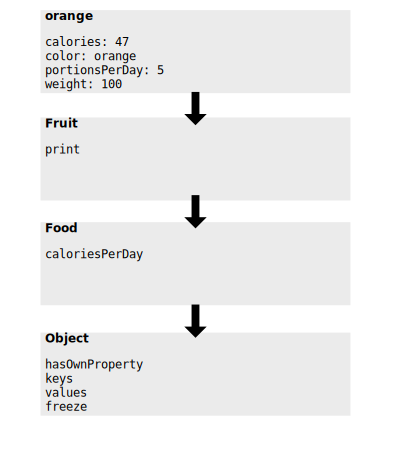
\includegraphics[width=10cm]{prototypechain} 
}
\caption{\label{fig:fig:js-prototypal-chain} Prototypal Inheritance in JavaScript.}
\end{figure} 

\subsection{Arrays}
Unlike other languages, JavaScript does not model arrays as continuously indexed tuples. Instead arrays are  a special form of object where array elements are properties that satisfy the following test for a key ToString(ToUint32(k)) === k \&\& ToUint32(k) !== 2 \textasciicircum 32 - 1). In simpler terms, an array is a special case of an object where the array elements are any value where the property can be coerced to a a positive integer number less than 2\textasciicircum32\textasciicircum - 1. These array elements are treated differently to regular properties by array prototypes and the length property. 

The length of an array is a property of the array prototype which tracks the highest index in the array. Note, that the highest index of the array does not necessarily track the number of elements in the array as arrays do not enforce any kind of ordering on their properties making it possible to create a non-contiguous array, an array with 'holes' in it, as shown in the example in figure \ref{fig:js-array-length}. The length product is not read-only as you might expect. If you increase length empty elements will be added to the end of the array and decreasing the length will truncate the array to satisfy the new length.

\begin{figure}[h]
\begin{verbatim}
let arr = [] // an empty array
arr[0] = 0
arr[2] = 2
$ arr
< [0, , 2]
$ arr.length 
< 3
\end{verbatim}
\caption{\label{fig:js-array-length} Example of Array Length Behaviour}
\end{figure}

Another by-product of arrays being a special form of object is that arrays are not homogenously typed. Whilst most languages require arrays to only hold values of a single type, JavaScript objects and by extension arrays can contain multiple types of value as shown by the following example let array = ['a', 2.0, \{\}, new Fruit()]. 

As described above, arrays can have both properties and array elements. If the property fails the array element test described above, then the value is stored as a regular object value. This can lead to subtle bugs when working with numbers if bounds are not checked as values smaller than 0 and greater than 2\textasciicircum32\textasciicircum - 1 will not be stored as an array element, as demonstrated in \ref{fig:js-array-max-length}.

\begin{figure}[h]
\begin{verbatim}
let arr = []
arr[0] = 'foo' // array element
$ arr.length
> 1
arr[4294967296] = 'bar' // 4294967296 === 2\textasciicircum32-1, property not an element
arr[-1] = 'baz' // -1 < 0, property not an element
$ arr.length
> 1
$ arr[4294967296]
> 'bar'
$ arr[-1]
> 'baz'
\end{verbatim}
\caption{\label{fig:js-array-max-length} Example of Array Object Behaviour }
\end{figure}

\subsection{Prototype Methods}
The array prototype has a large number of helper functions which developers frequently take advantage of, a number of which were added in the latest version of the EMCAScript standard~\cite{EcmaScript}. \ref{table:array-prototype} has some of the more commonly used and interesting functions.
\afterpage{%
    \clearpage% Flush earlier floats (otherwise order might not be correct)
    \begin{landscape}% Landscape page
\begin{table}[h]
\centering
\caption{Array Prototype Methods}
\label{table:array-prototype}
\scalebox{.53}{
\begin{tabular}{|l|l|l|}
\hline
Function Name & Signature & Description \\ \hline
indexOf &indexOf(element) & Returns the first index of the array that containselement or -1 ifelement is not in the array \\ \hline
lastIndexOf &lastIndexOf(element) & Returns the last index of the array that containselement or -1 if element is not in the array \\ \hline
slice &slice(begin, end) & Returns a copy of the array with the elements from the indexbegin up to theend index. Ifend is not provided it will slice frombegin to the last element of the array \\ \hline
push &push(element) & Increases the length of the array by one and addselement to the end of the array \\ \hline
pop &pop() & Removes the last element in the array and returns it \\ \hline
unShift &unShift(elementA, elementB, ...) & Adds one or more elements to the beginning of an array and returns the new length \\ \hline
includes &includes(element, startIndex) & Returns true if the array contains element either starting fromstartIndex or the start of the array if no startIndex is provided \\ \hline
reverse &reverse() & Reverses the array in place and returns a reference to the array \\ \hline
forEach &forEach(func) & Callsfunc on each element in the array. Callsfunc with(value, index, array) \\ \hline
filter &filter(func) & Returns a new array that contains elements that return true whenfunc is called on them.func is called withcurrentElement \\ \hline
map &map(func) & Returns a new array with the results of callingfunc on each element in the array.func is called with(value, index, array) \\ \hline
reduce &reduce(func, initialValue) & Callsfunc(accumulator, value, index, array) on every element in the array and returns the value of accumulator. IfinitialValue is provided then the first timefunc is called thenaccumulator is set to the value ofinitialValue \\ \hline
some &some(func) & Callsfunc(element, index, array) for every element in the array. Returns true iffunc returns true for at least one element in the array \\ \hline
every &every(func) & Calls func(element, index, array) for every element in the array. Returns true iffunc returns true for all elements in the array \\ \hline
\end{tabular}
}
\end{table}
\end{landscape}
    \clearpage% Flush page
}


\section{Ensuring the Correctness of JavaScript}
As described in 1.1, assuring the correctness of JavaScript code is an unsolved problem - in part due to the fact JavaScript is a dynamically typed scripting language but also due to legacy design decisions. Efforts have been made to make the language itself safer to use, for example ECMAScript 5 introduced a strict mode (later made the default mode in ECMAScript 6) which restricts the use of certain language features and also defines additional circumstances that exceptions should be thrown. However there are still many subtle errors that can occur even within the safer subset of JavaScript.

Tools like Eslint and Flow are commonly used by developers to statically analyse code and identify bugs but are limited in their scope. Eslint uses a narrow set of rules to identify possibly dangerous behaviour and Flow is constrained to reasoning about types and in some cases requires additional code annotation to allow Flow to identify possible errors. These limited sets of warnings do not fully reflect the dynamic nature of JavaScript and the subtle interactions that can occur due to prototypical inheritance, dynamic property access, and dynamic dispatch. There have been a number of attempts to analyse JavaScript statically however most approaches fall short of useful due to their inability to reason about functions like\lstinline{call()} and \lstinline{apply()}~\cite{sridharan2012correlation} with the best results requiring an element of dynamic analysis as well~\cite{logozzo2010rata, wei2013practical}.

Consequently there has been a shift in interest towards analysing safer (and less dynamic) targets which compile to JavaScript, the most popular of which is Typescript. Typescript is a superset of ECMAScript 6 which includes optional types to enable errors to be caught statically before compilation. Although TypeScript makes it easier to reason about potential errors caused by coercion, TypeScript itself provides no guarantees of static soundness - it's still possible for a TypeScript program to compile to JavaScript successfully and encounter a run-time error as a result of type coercion when executed~\cite{bierman2014understanding}. Extensions to TypeScript have been suggested to provide soundness ~\cite{richards2015concrete, rastogi2015safe} although these approaches require a modified interpreter or runtime enforcement. Regardless, whilst TypeScript and its derivatives provide a way of reducing or eliminating type based errors they don't help identify or eliminate errors that occur due to other dynamic features of JavaScript such as prototypical inheritance, dynamic property access, or dynamic dispatch.

There have been a number of attempts to produce formal semantics for JavaScript, to allow for better reasoning about JavaScript code, however no attempts can be considered completely successful. One approach taken by Gardner et al. (JaVerT) ~\cite{gardner2012towards, guha2010essence} is to translate a subset of the JavaScript language (targeting ECMAScript 5 in strict mode) to an intermediate language, JSL, and then performing analysis on JSL. Although the results of their analysis with translated code is promising, their process and toolchain requires an expert level understanding of the semantics of JavaScript and developers to annotate their code pre and post-conditions. Although, this approach may be suited for smaller programs (or critical subsets of programs) its approach does not scale well to large applications. Other approaches such a KJS~\cite{park2015kjs} and λJS~\cite{guha2010essence} support even less of the language than JaVerT and crucially none of the three approaches target the ECMAScript 6 specification.

Symbolic execution provides an ideal way to test JavaScript code. By concretely executing the program, reasoning about the dynamic nature of JavaScript is deferred to the interpreter. The use of an interpreter for testing also provides flexibility. If JavaScript needs to be tested in another environment, switching interpreter is a relatively easy change to make. Additionally, concrete execution comes without the penalty of having to model the entire language specification as any non-modelled function can simply revert to concrete execution. Finally, symbolic execution is also able to test any JavaScript underlying library code.

ExpoSE is a tool for symbolic execution of JavaScript. The target program is instrumented with Jalangi2, a tool that provides hooks before and after each statement is executed, which is used to build a symbolic representation of the program. ExpoSE uses a harness to randomly generate inputs for public functions in a target JavaScript program. It then uses a DART~\cite{godefroid2005dart} based directed search to attempt to explore all feasible paths in the program up to a maximum path count.

\chapter{Implementation Details}
Z3, the SMT solver used by ExpoSE, supports two array-like theories: the theory of arrays, and the theory of sequences which provided a choice for which theory to encode JavaScript arrays in. The Z3 offers a rich number of methods for sequences including obtaining the length, concatenating sequences, and checking whether an element is in a sequence. Contrasting, the theory of array support is limited to two operations: select and store. Consequently, sequences seemed like a more natural fit to encode JavaScript arrays as many array prototype methods map naturally to Z3 sequence functions. For instance,\lstinline{Z3_mk_seq_contains} is equivalent to \lstinline{Array.prototype.includes} and \lstinline{Z3_mk_seq_index} is equivalent to to \lstinline{Array.prototype.indexOf}. However after experimentation it became clear that concretising sequences was impossible as extracting single elements from a sequence produced a unit sequence rather than the value of the element. As a result of being unable to concretise sequences, JavaScript arrays are encoded using Z3’s array theory.


Z3 arrays are one dimensional unbounded maps where the index and values are of any given sort. Read and write operations on the array are mapped to select and store axioms respectively. The SMT logic below demonstrates the basic relationship between store and select.

\begin{figure}[t]
\begin{verbatim}
(declare-const i Int)
(declare-const v Int)
(declare-const a (Array Int Int))
(assert (= (store a i v) a))
(assert (= (select a i) v))
(check-sat)
(get-model)
\end{verbatim}
\caption{\label{fig:z3-select-store} Example of Select and Store Axioms in Z3 Arrays}
\end{figure}

TODO REWRITE EVERYTHING BELOW THIS IN THIS CHAPTER AFTER SLICE IS IMPLEMENTED (INCLUDING CODE EXAMPLES!)

Due to way Z3 models arrays as a unbounded homogeneously typed data structure, Z3 arrays do not directly correspond to JavaScript arrays. In order to encode the finite length of JavaScript arrays a separate Z3 integer variable is used which represent the the length of the symbolic array. When the array is created an assertion is made that the length is greater than or equal to 0. Whenever the concrete JavaScript array is accessed, if the index of the array is less than the concrete length of the array then an assertion is made that the symbolic length is less than the accessed index - else an assertion is made that length is greater than or equal to the accessed index.

\begin{figure}[h]
\begin{verbatim}
// field_c is the concrete field accessed, base_c is the concrete array, base_s is the symbolic array, field_s is the symbolic field accessed
 if (field_c >= base_c.length) {
    this.pushCondition(this.ctx.mkGe(field_s, base_s.length))
    return undefined
 } else {
    this.pushCondition(this.ctx.mkLt(field_s, base_s.length))
     return base_s.selectFromIndex(this.ctx.mkRealToInt(field_s))
}
\end{verbatim}
\caption{\label{fig:expose-get-field} Example of Array Constraints Enforcement}
\end{figure}

When the array is manipulated by push() and pop() operations the Z3 length variable is replaced by a new variable where the length is greater than or less than the previous array length respectively. As array values in Z3 can only be of one type and JavaScript arrays are non-homogenous only homogenously typed arrays can be symbolically represented.

\section{Array Support Architecture}
ExpoSE is architected as a number of distinct modules: Z3JS, a JavaScript interface to Z3’s C API, the Distributor, a highly parallelised dispatcher for symbolic execution paths and an aggregator of information, the Analyser, which performs the symbolic analysis for a given path, and the Tester, which automatically runs ExpoSE’s unit tests. The bulk of my work, outlined below, was done in the Analysers and Z3JS. I’ll briefly outline the modifications that were made to each.

\subsection{Analyser}
SymbolicState.js has a number of callbacks that are called when a symbolic value is used during execution. \lstinline{createSymbolicValue()} has been modified to check if the concrete type is either homogeneously typed or empty array, if so Z3JS’s \lstinline{context.mkArray()} is called to create the array, with the correct homogenous type, and assertions are made about the array’s length, as described above, to keep the array bounded. 

\lstinline{symbolicField()} has been modified to check if the array is being accessed with a potentially valid array index - i.e. a number between 0 and 2\^32-1. If so, assertions are made about the length, as described above, and if the index is less than the array length Z3JS’s \lstinline{Expr.selectFromIndex()} is called. When an array’s length is accessed the expression for the array length is returned.

In order to symbolically model the behaviour of prototype functions the Analyser has a module, Function Models, which contains a symbolic hook that concretely executes the function and then if a condition is met also symbolically executes a model function if it exists.  I’ve added prototype functions for a number of commonly used Array prototypes, such as a \lstinline{push()} and \lstinline{indexOf()}.

TODO Expand on an individual prototype function (perhaps includes - SMT notation to Z3JS symbolic hook with a line by line breakdown of what’s actually going on

\subsection{Z3JS}
Z3JS provides an interface between the Z3’s C API and JavaScript. It’s main components are a Solver class, a Query class, a Model class, an Expr class, and a Context class. The context class wraps the Z3 context and acts as a facade for the Z3 API calls. The Expr class wraps constructed Z3 expressions and has helper functions for printing and creating a concrete value from the symbolic expression. The model class wraps Z3 model objects and the query class is used to request solutions for models from Z3.

In order to be able to interface with Z3’s array functions I had to add a number of functions to the context class including \lstinline{mkArray}, \lstinline{mkSelect}, \lstinline{mkStore} as well as functions used to perform assertions using quantifiers, \lstinline{mkForAll} and \lstinline{mkExists}. The quantifier based functions expect arrays to be passed as parameters so I also had to change some helper functions \lstinline{_buildChecks()} and \lstinline{Z3Utils.astArray()} to work with arrays of parameters.

The key function in Expr is asConstant() which turns the expression into a concrete value. I rewrote the function into a small switch statement which evaluates the sort of the expression. To be able to support turning array expressions into constants I had to be able to get a constant value for the expression which represents the length of the array. In order to do that I had to change the signature of the function to accept a model, using which I can call \lstinline{model.eval()} to get an interpretation for the expression. Using the concrete value for the length I can then iterate for the length of the array calling \lstinline{selectFromIndex()}, a helper function in Expr which calls context.mkSelect for a given index, to produce a concrete JavaScript array of values.

I also use Expr to hold two properties which are specific to arrays, the length expression and the name of the array.

\subsection{Other Interesting Engineering Techniques}
Each array functionality is backed by one or more tests. Each test has an expected number of symbolic paths which should be produced an expected number of errors so regressions in behaviour can be identified. Array support can be disabled in the analyser through the use of an environment variable. This allows programs to be executed with and without array support so that behaviour and coverage can be compared.


\chapter{Results}

TODO

A deep dive into one specific program (?) with cases not caught
An overall comparison with array support on/off on a large number of targets
Prototype usage

\section{Conclusion}

\newpage
\bibliography{/Users/arran/Documents/Github/FullUnit_1718_ArranFrance/Report/bibliography}
\bibliographystyle{ieeetr}
\label{endpage}



\end{document}

\end{article}
